\chapter{\textit{Onboarding}}\label{cap3}

Aqui descrevo o meu breve processo de Onboarding. O qual passou pelo primeiro dia onde foi a parte administrativa, e posteriormente a parte formativa onde durante duas semanas estive a ser preparado para o projeto.

\section{O que é Onboarding?}

Em linhas gerais, onboarding trata-se de um processo para integrar o novo membro à equipa, cultura e forma de operação da empresa, com o objetivo de assegurar a adaptação e a retenção deste profissional.

É o processo de integração de novos empregados numa empresa, para que eles possam obter os conhecimentos, as habilidades e os comportamentos necessários a fim de efetivamente se tornarem parte da equipa.

Envolve várias etapas, que podem ser conjuntas ou separadas, como orientação, supervisão, acompanhamento e treinamento, por exemplo.

\section{Fase Administrativa}

Chamo de fase administrativa ao primeiro dia de estágio, este dia passou pela introdução informal do local de estágio, as regras de trabalho, as normas de segurança e o que é necessário para o bom desenvolvimento do projeto.

Foi também neste dia que me foi atribuído a conta empresarial (backend da Google), com email, senha e perfil de acesso, como também o que esta conta oferece (tal como drive, sheets, etc).

Essa conta base serve também para login na conta da Atlassian, onde tenho acesso a todas as ferramentas de estágio, como o Jira, Confluence, Bitbucket, etc.

Finalmente foi feita uma reunião, comigo e com todos os outros estagiários (três alunos da Universidade de Évora, sendo que um também é um estagiário de Backend), para nos passar à fase formativa, onde estarei a desenvolver competências base para o projeto.

\newpage

\section{Fase Formativa}

Esta fase teve uma duração base de duas semanas. Aqui foi-nos doado três cursos do \href{https://www.udemy.com/}{Udemy}, gradualmente e sequencialmente dependendo do progresso do estagiário.

Estes cursos tinham como objetivo ajudar ao estagiário a desenvolver competências para o projeto que será desenvolvido, o qual reflete as competências que o estagiário deve possuir para poder trabalhar no backend da empresa que está a trabalhar.

O primeiro curso foi \href{https://www.udemy.com/course/build-reactive-restful-apis-using-spring-boot-webflux/}{\textit{``Build Reactive MicroServices using Spring WebFlux/SpringBoot''}}, que têm como objetivo ensinar a fazer backends de serviços, ou micro serviços em Spring, mas com uma particularidade: usar \href{https://spring.io/reactive}{Spring WebFlux} que é a implementação da \href{https://spring.io/}{Spring} do \href{https://projectreactor.io/}{Project Reactor}. Isto permite fazer uma API reativa, ou seja, uma API que é capaz de receber requisições e retornar respostas de forma assíncrona e com a menor latência possível.

\begin{figure}[!hbt]
  \centering
  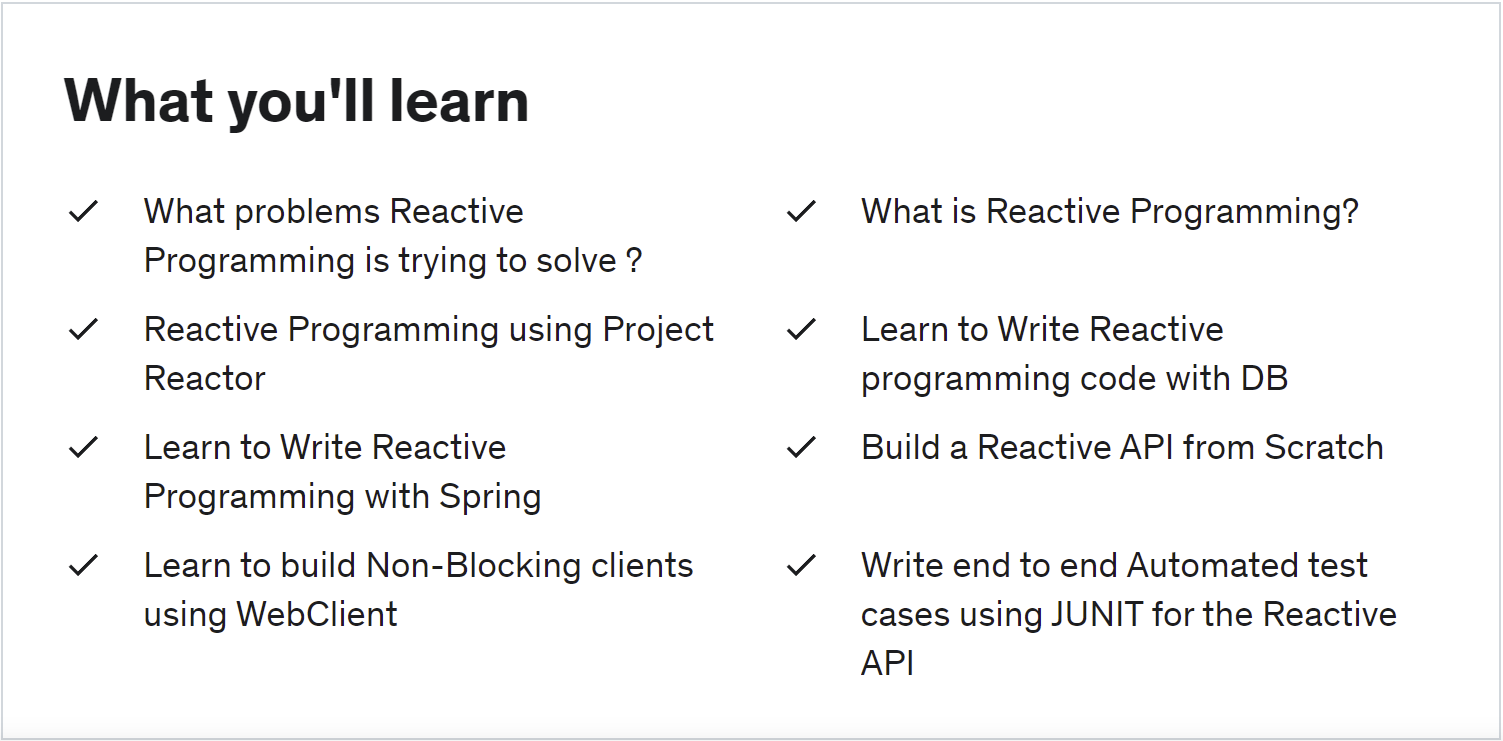
\includegraphics[width=14cm]{figuras/udemy1.png}
  \caption{Conteúdo do curso \textit{``Build Reactive MicroServices using Spring WebFlux/SpringBoot''} do \href{https://www.udemy.com/}{Udemy}}
  \label{fig:udemy1}
\end{figure}
\FloatBarrier

Seguidamente foi-me destacado o \href{https://www.udemy.com/course/grpc-the-complete-guide-for-java-developers/}{\textit{``Microservices with gRPC [Java + Spring Boot + Protobuf]''}}, que é um curso com o objetivo de ensinar ao estagiário a desenvolver \textit{microservices} com \href{https://grpc.io/}{gRPC} em \href{https://jdk.java.net/}{Java} usando \href{https://developers.google.com/protocol-buffers}{Protocol Buffers}, ou seja, um serviço que usa a implementação de RPC da \href{https://abc.xyz/}{Google} e usa o \href{https://developers.google.com/protocol-buffers}{Protocol Buffers} para o transporte de dados. Isto têm a vantagem de ser um serviço de baixo custo, e alta velocidade de comunicação.

\begin{figure}[!hbt]
  \centering
  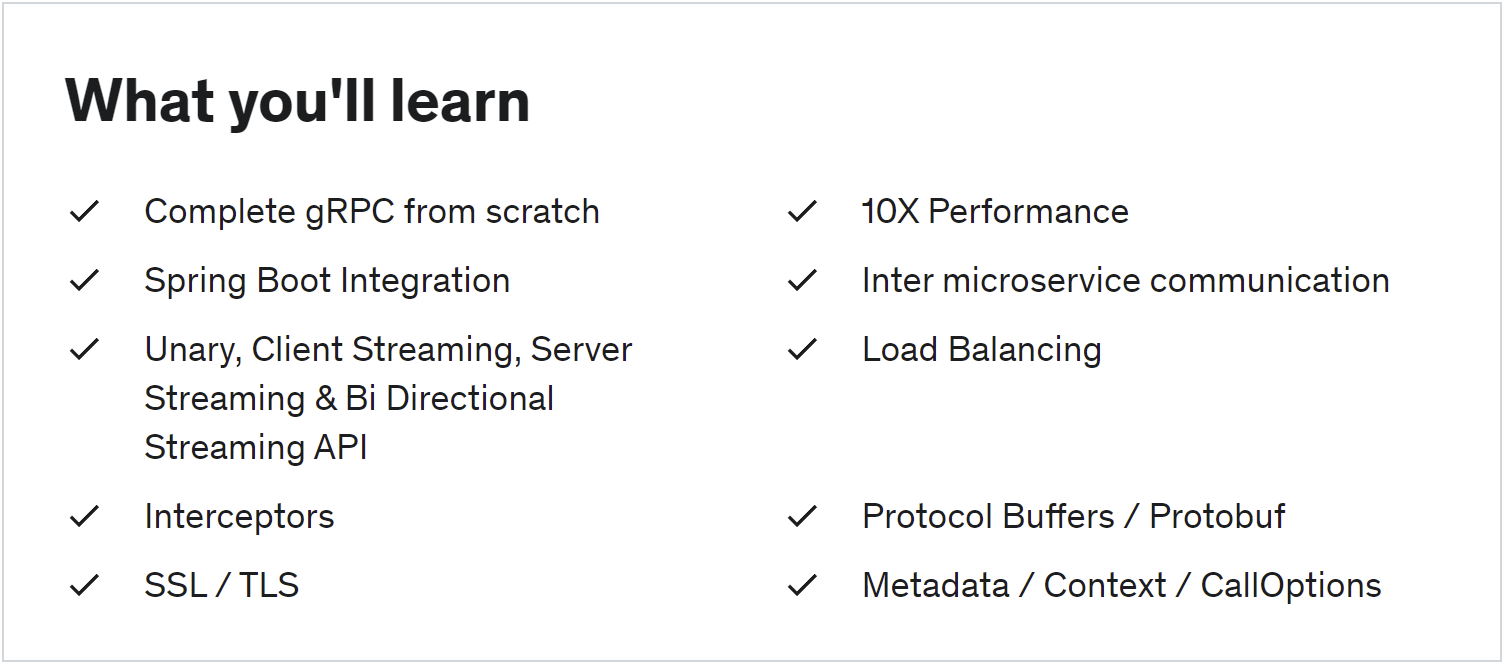
\includegraphics[width=14cm]{figuras/udemy2.png}
  \caption{Conteúdo do curso \textit{``Microservices with gRPC [Java + Spring Boot + Protobuf]''} do \href{https://www.udemy.com/}{Udemy}}
  \label{fig:udemy2}
\end{figure}
\FloatBarrier

O ultimo curso foi o \href{https://www.udemy.com/course/learn-micronaut/}{\textit{``Learn Micronaut - cloud native microservices with Java''}}, que nos mostra como fazer \textit{microservices} em Micronaut, um framework de \href{https://jdk.java.net/}{Java}, como o Spring mas com o objetivo de ser mais leve, modular e escalável. Este curso também passa pela integração do \href{https://kafka.apache.org/}{Apache Kafka}, um \textit{message broker} que permite a comunicação entre \textit{microservices} e como exportar o projeto para um \textit{native binary} e como usar o \href{https://www.graalvm.org/}{GraalVM}, que é uma JVM de nova geração, mais leve e mais rápida que também suporta outras linguagens de programação.

\begin{figure}[!hbt]
  \centering
  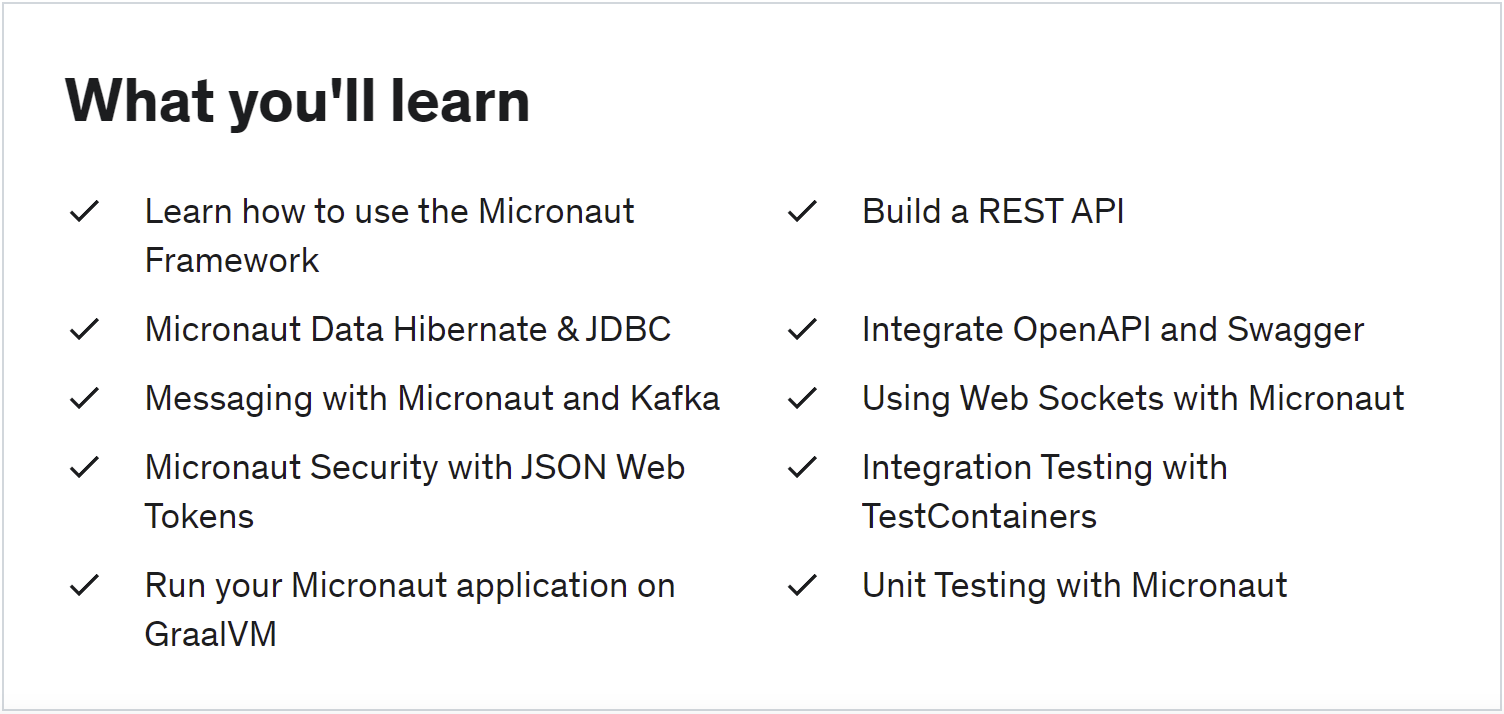
\includegraphics[width=14cm]{figuras/udemy3.png}
  \caption{Conteúdo do curso \textit{``Learn Micronaut - cloud native microservices with Java''} do \href{https://www.udemy.com/}{Udemy}}
  \label{fig:udemy3}
\end{figure}
\FloatBarrier
